VR Training bei Bodenfahrzeugen
Bei Autorennen werden VR-Simulatoren verwendet, die meist auch Lenkrad und Pedale mit beinhalten. Die meisten Rennfahrer benutzen diese um sich Rennstrecken einzuprägen und diese zu fahren. Jedoch ist das Training populärer bei Hobby-Rennfahrern als bei Professionellen Rennfahrern, da die Professionellen von ihrem Verein Trainingstrecken und Rennautos gestellt bekommen und dies natürlich ein besseres Training ist, da sie dabei ein zu eins das machen was sie trainieren. Bei dem VR Simulatoren fehlen meist bestimmte Einflüsse wie physische Störungen oder das Momentum, das auf den Körper übertragen wird beim Bremsen beziehungsweise Beschleunigen. Für Hobby-Sportler ist der VR-Simulator eine günstige und einfache Alternative auf berühmten Rennstrecken und sehr teuren Rennwägen zu fahren.
\\
\begin{figure}[!ht]
    \centering
    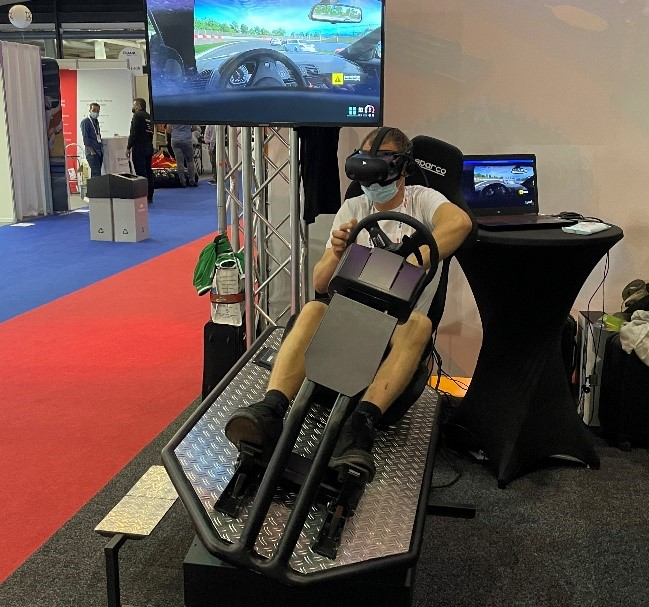
\includegraphics[width=1.0\textwidth]{images/Abbildung 2.jpg}
    \caption{\label{fig:Abbildung 2}Autorenn-Simulator (full-motion)\protect
    }
\end{figure}
Derzeitig wird jedoch auch an normalen Autofahr-Simulatoren (für Führerscheine) mit VR geforscht. Diese könnten bei Fahrlehrlingen die grade ihren Führerschein machen helfen, da wie auch bei den Rennsimulatoren kein echtes Auto und keine echte Straße benötigt wird. Das gibt die Vorteile in keine gefährlichen Situationen zu geraten, andere in keine gefährlichen Situationen zu bringen und die Kosten sind um einiges billiger. Dazu kann man mit verschiedenen Autos Trainieren. Am hilfreichsten ist der Autofahr-Simulator den Fahrlehrling zu trainieren was dieser in Stress- und Panik-Situationen macht ohne irgendein Risiko einzugehen \cite{ihemedu2017virtual}. Zusätzlich kann der Fahrlehrling Mut und Selbstsicherheit aufbauen währenddessen er im Simulator fährt und keine Fehler baut. Nachteile sind, dass man das Gefühl des Autofahrens nicht direkt übermittelt bekommt, dadurch können Sachen wie die Kupplung richtig benutzen und auch gefühlsvoll zu bremsen nicht wirklich durch den Simulator erlernt werden.
\\
\begin{figure}[!ht]
    \centering
    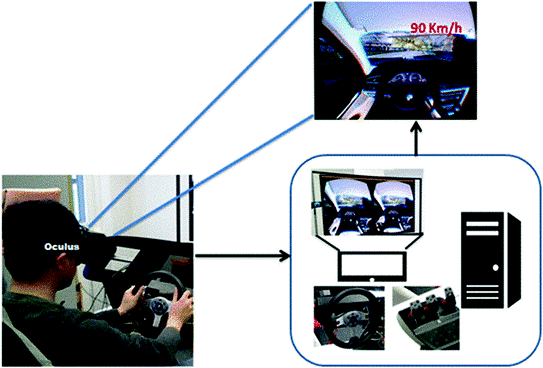
\includegraphics[width=1.0\textwidth]{images/Abbildung 3.png}
    \caption{\label{fig:Abbildung 3}Beispiel wie VR bei einer Fahrschule eingesetzt werden könnte\cite{ihemedu2017virtual}\protect
    }
\end{figure}
\\
Bei Bodenfahrzeugen ist VR-Training im Bereich der Rennautos weit entwickelt und wird von vielen benutzt, sogar von nicht-Sportlern, die einfach nur Spaß an einem VR-Spiel haben. Bei dem Trainieren von dem Auto fahren selbst ist die VR-Technologie noch kaum angekommen, aber es gibt positive Ausblicke das auch in diesem Teilbereich die VR-Technologie integriert wird und somit es leichter macht.

Abbildung 2 \footnote{\url{https://eveprocom.de/eventmodule/virtual-reality/full-motion-vr-racing-seat-pro-mieten/}}

